拉伸建模法是通过绘制物体的底面的特征平面,然后利用此平面沿轴线方向堆叠来构建物体模型的方法。由此可知,杯零件不的三维模型不仅可以用旋转建模法也可以用拉伸建模法。本节将用拉伸建模法构建杯零件的三维模型。
\subsection{绘制杯零件主视图}
通过观察,杯零件的主视图清晰地表达了其底面特征,要使用拉伸建模法就需要绘制杯块零件的主视图。
\begin{procedure}
\item 将视图切换为主视图。
\item 绘制圆。

启动【圆】命令的方法有:
\begin{itemize}
\item 键盘输入CIRCLE\index{circle} 或C。
\item 【绘图】$\rightarrow$【圆】$\rightarrow$【圆心、半径】。
\item 【绘图】$\triangleright$【圆】图标
\includegraphics[scale=0.6]{circletool.png}。
\end{itemize}

绘制$\phi 30$的圆。
启动【圆】命令后,要求输入圆的圆心位置。
\begin{figure}[htbp]
\centering
\subfloat[]{\label{fig:centerselect}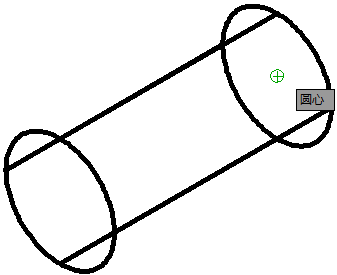
\includegraphics[scale=0.5]{centerselect.png}}\hspace{20pt}
\subfloat[]{\label{fig:beifront}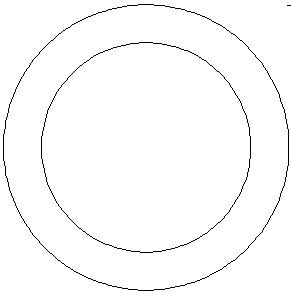
\includegraphics[scale=0.5]{beifront.png}}
\caption{杯零件主视图绘制}
\end{figure}
\begin{lstlisting}
|命令: CIRCLE|
|指定圆的圆心或 [三点(3P)/两点(2P)/切点、切点、半径(T)]: 15,15|
\end{lstlisting}
接下来输入圆的半径值。若要以直径方式输入,则需要使用D选项,再输入直径值。
\begin{lstlisting}
|指定圆的半径或 [直径(D)]: 15|
\end{lstlisting}
绘制$\phi 22$的圆。绘制$\phi 22$圆时,既可以使用坐标方式指定圆心,也可以使用圆心捕捉来获取$\phi 30$圆的圆心坐标。用圆心捕获取坐标的方法比较方便,且能够加速绘图,实际绘图中应用较多。圆心捕捉开启方法有:
\begin{itemize}
\item 键盘为输入CE。
\item 鼠标捕捉。开启鼠标捕捉圆心的方法与开启直线端点捕捉的方法基本一致,具体请参见第\pageref{fig:duixiangbuzuomen2}页开启端点捕捉的方法,此处不再赘述。
\end{itemize}
 此处,用如图\ref{fig:centerselect}所示的方法捕捉圆心。
\begin{lstlisting}
|命令:  CIRCLE|
|指定圆的圆心或 [三点(3P)/两点(2P)/切点、切点、半径(T)]:|
|指定圆的半径或 [直径(D)] $<15.0000>$: 11|
\end{lstlisting}

\end{procedure}

\endinput